\begin{figure*}[t]
\centering
\begin{minipage}[t]{0.32\textwidth}
  \centering
  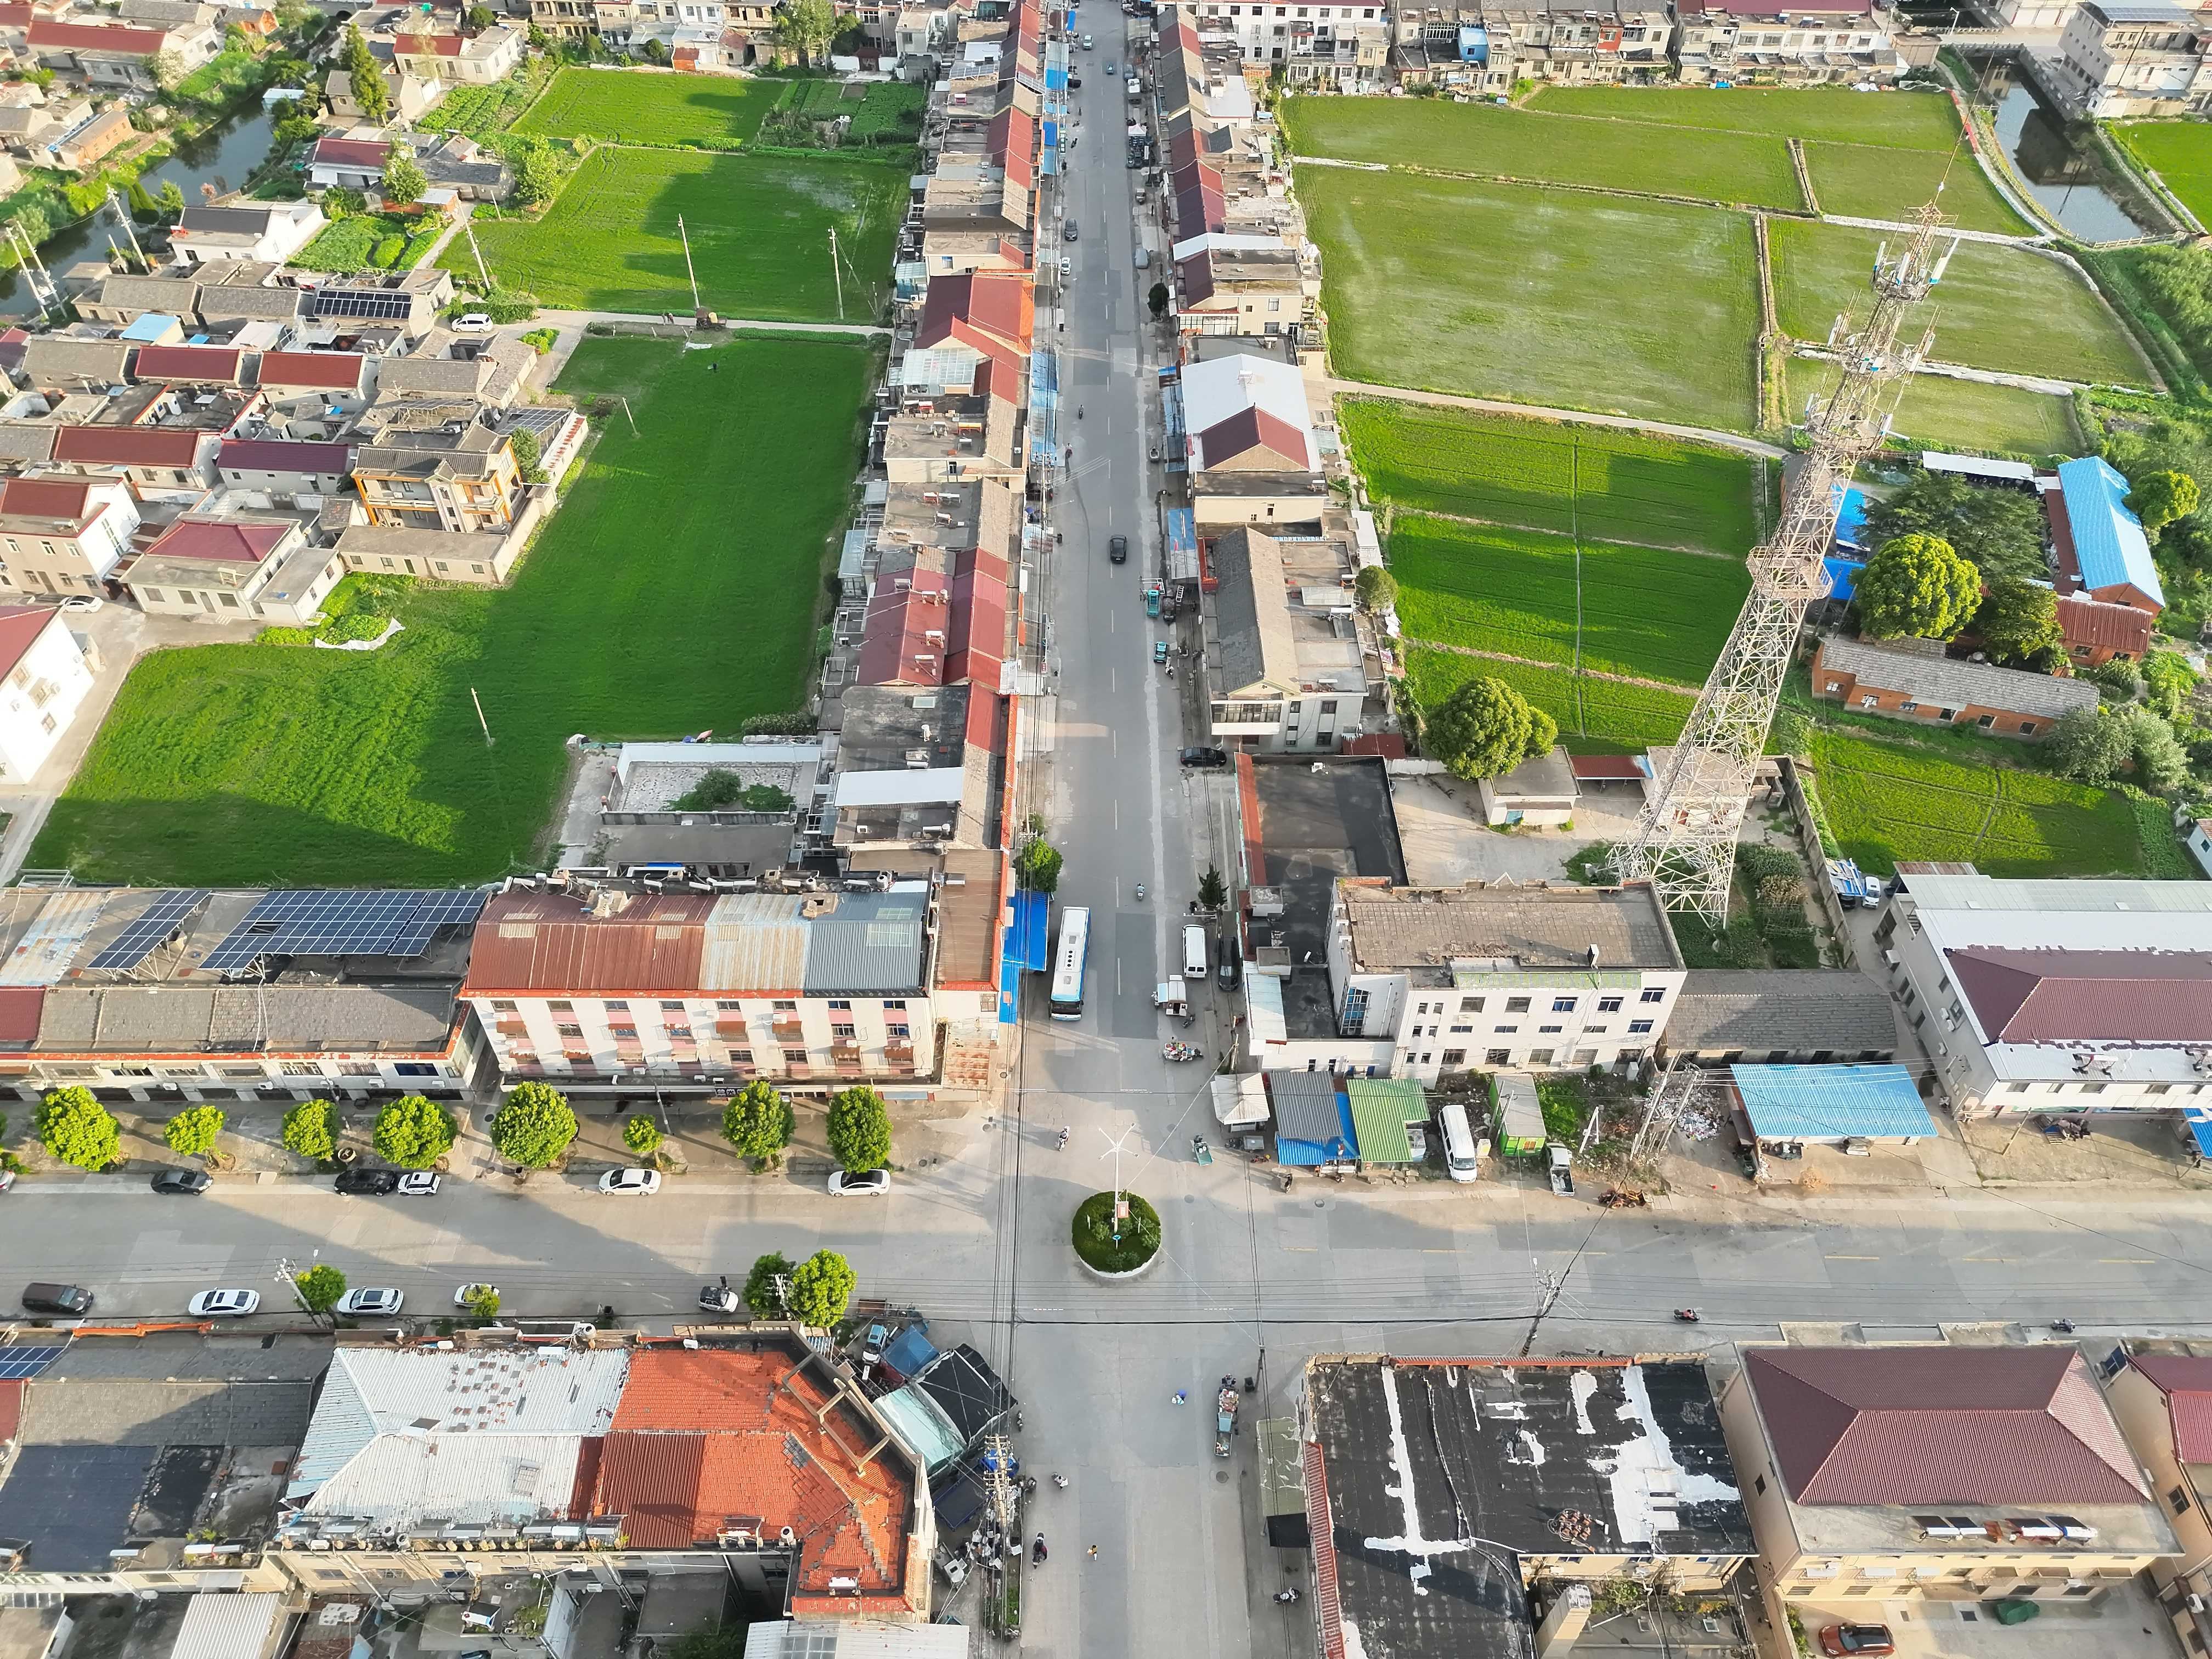
\includegraphics[width=0.61\linewidth,height=2.35cm,keepaspectratio]{street_vendor_context.jpg}\hfill
  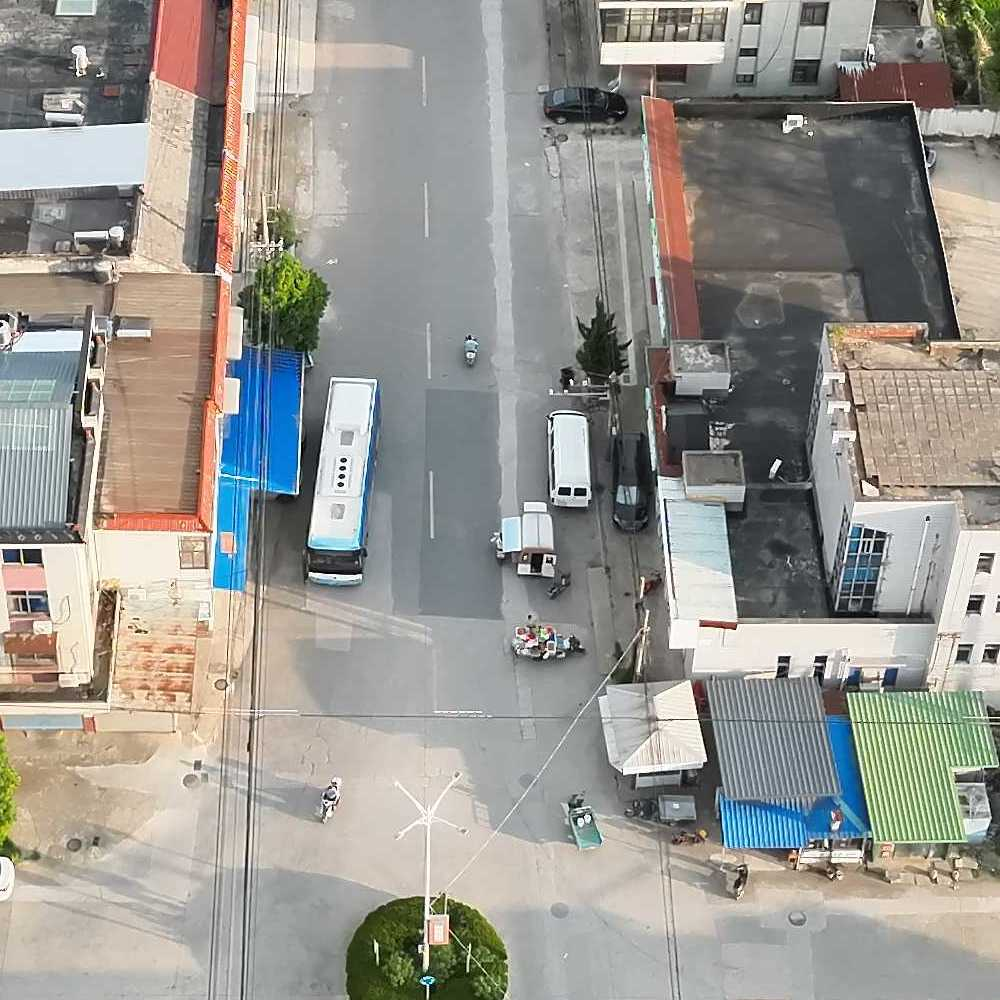
\includegraphics[width=0.37\linewidth,height=2.35cm,keepaspectratio]{street_vendor_evidence.jpg}
  \par\vspace{2pt}\footnotesize\textbf{(a) Street vendor.} Local identity plus roadway occupation.
\end{minipage}\hfill
\begin{minipage}[t]{0.32\textwidth}
  \centering
  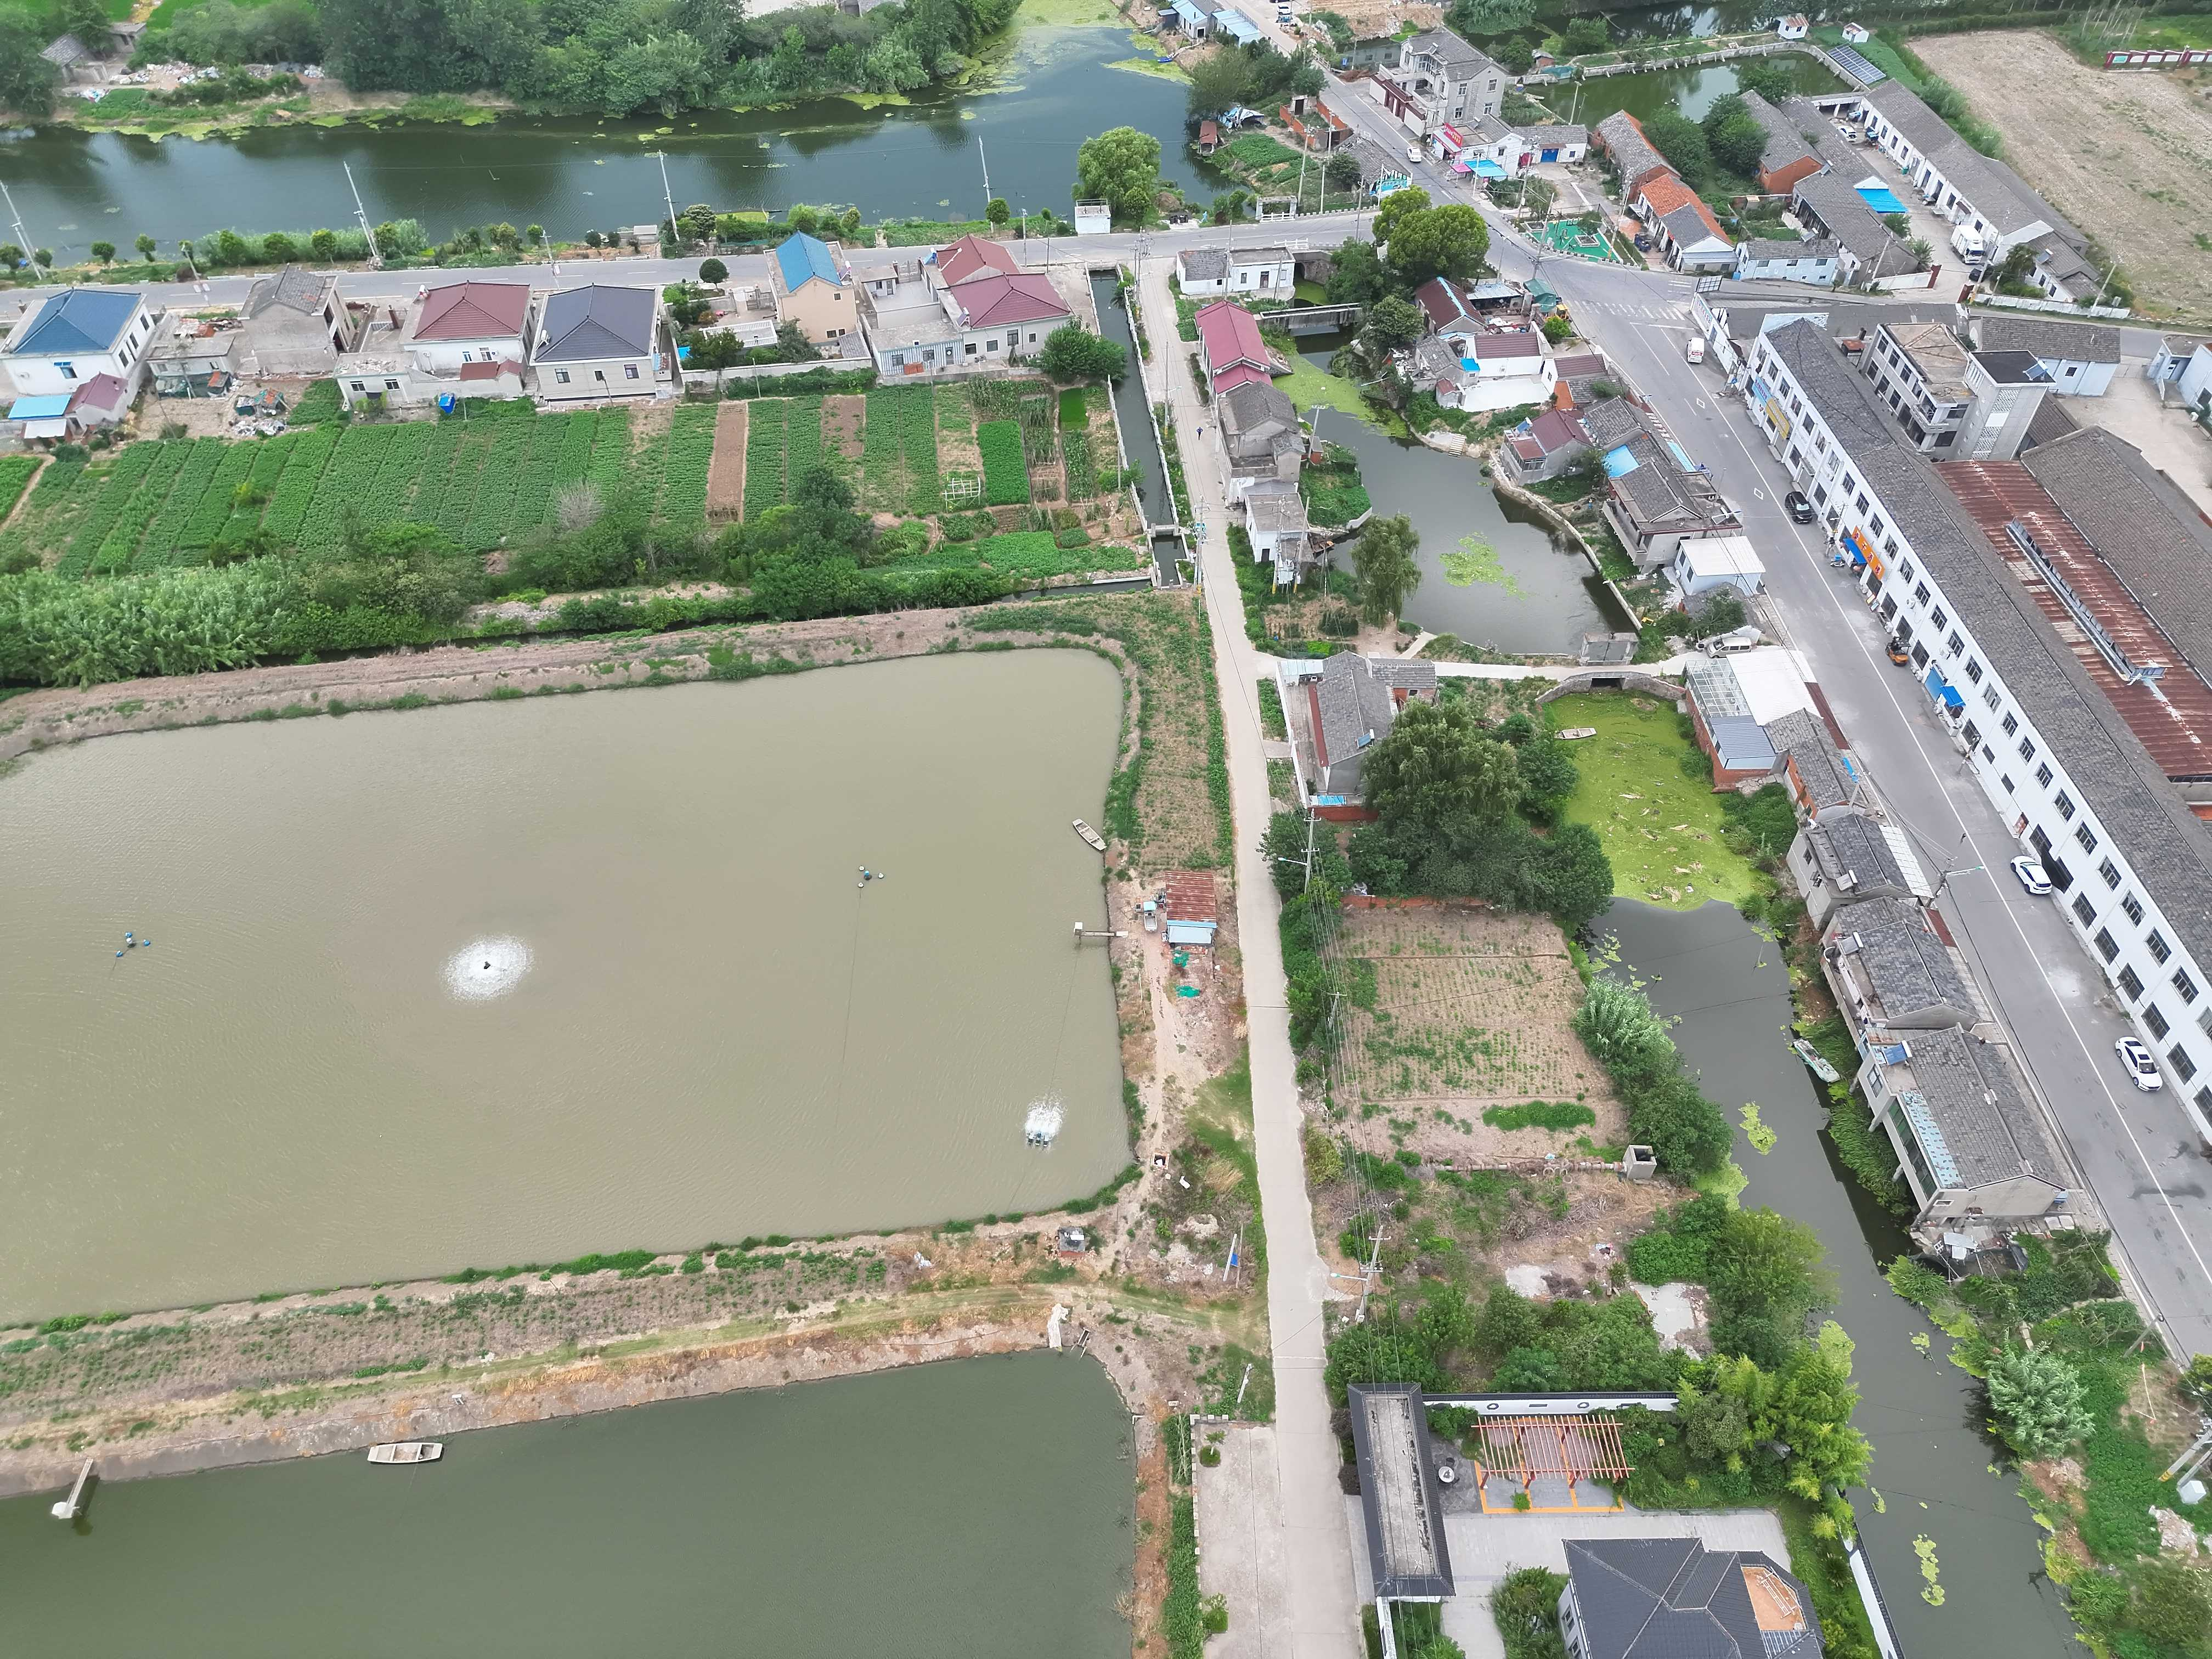
\includegraphics[width=0.61\linewidth,height=2.35cm,keepaspectratio]{floating_garbage_context.jpg}\hfill
  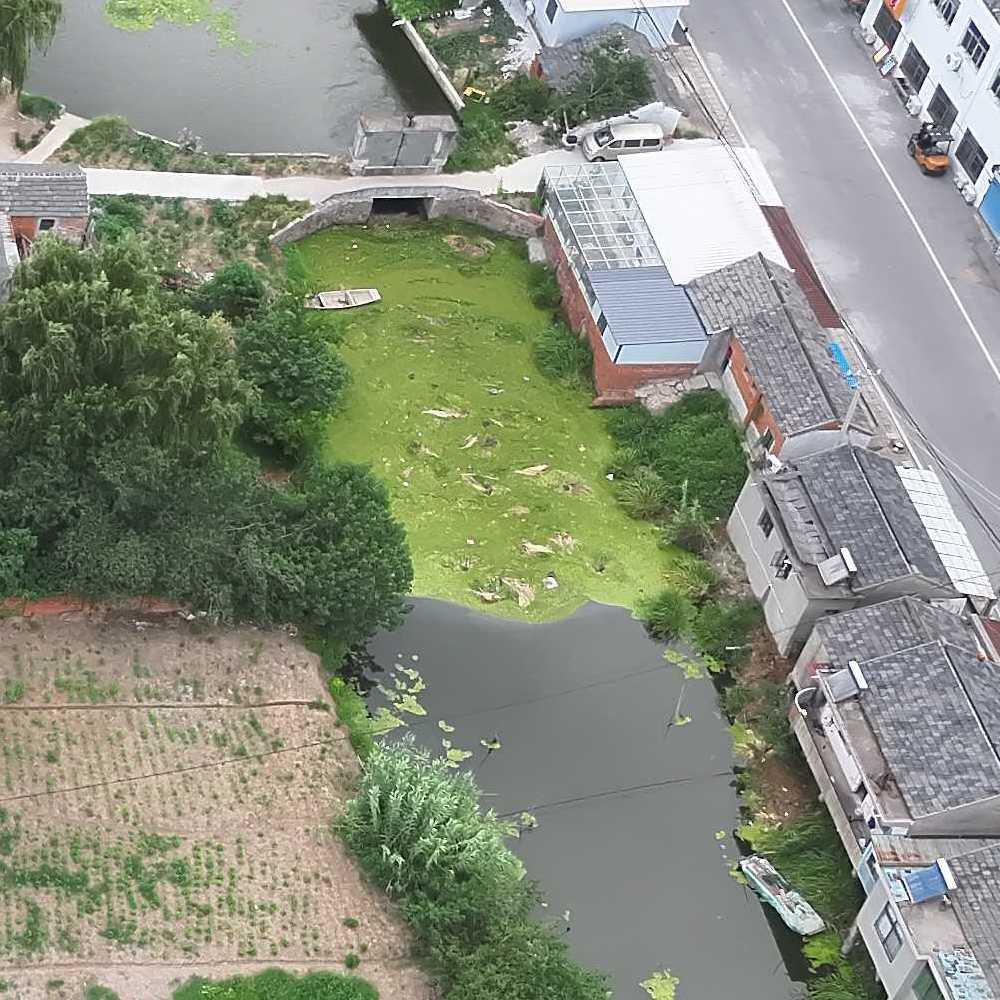
\includegraphics[width=0.37\linewidth,height=2.35cm,keepaspectratio]{floating_garbage_evidence.jpg}
  \par\vspace{2pt}\footnotesize\textbf{(b) Floating garbage.} Debris must lie on water, not the bank.
\end{minipage}\hfill
\begin{minipage}[t]{0.32\textwidth}
  \centering
  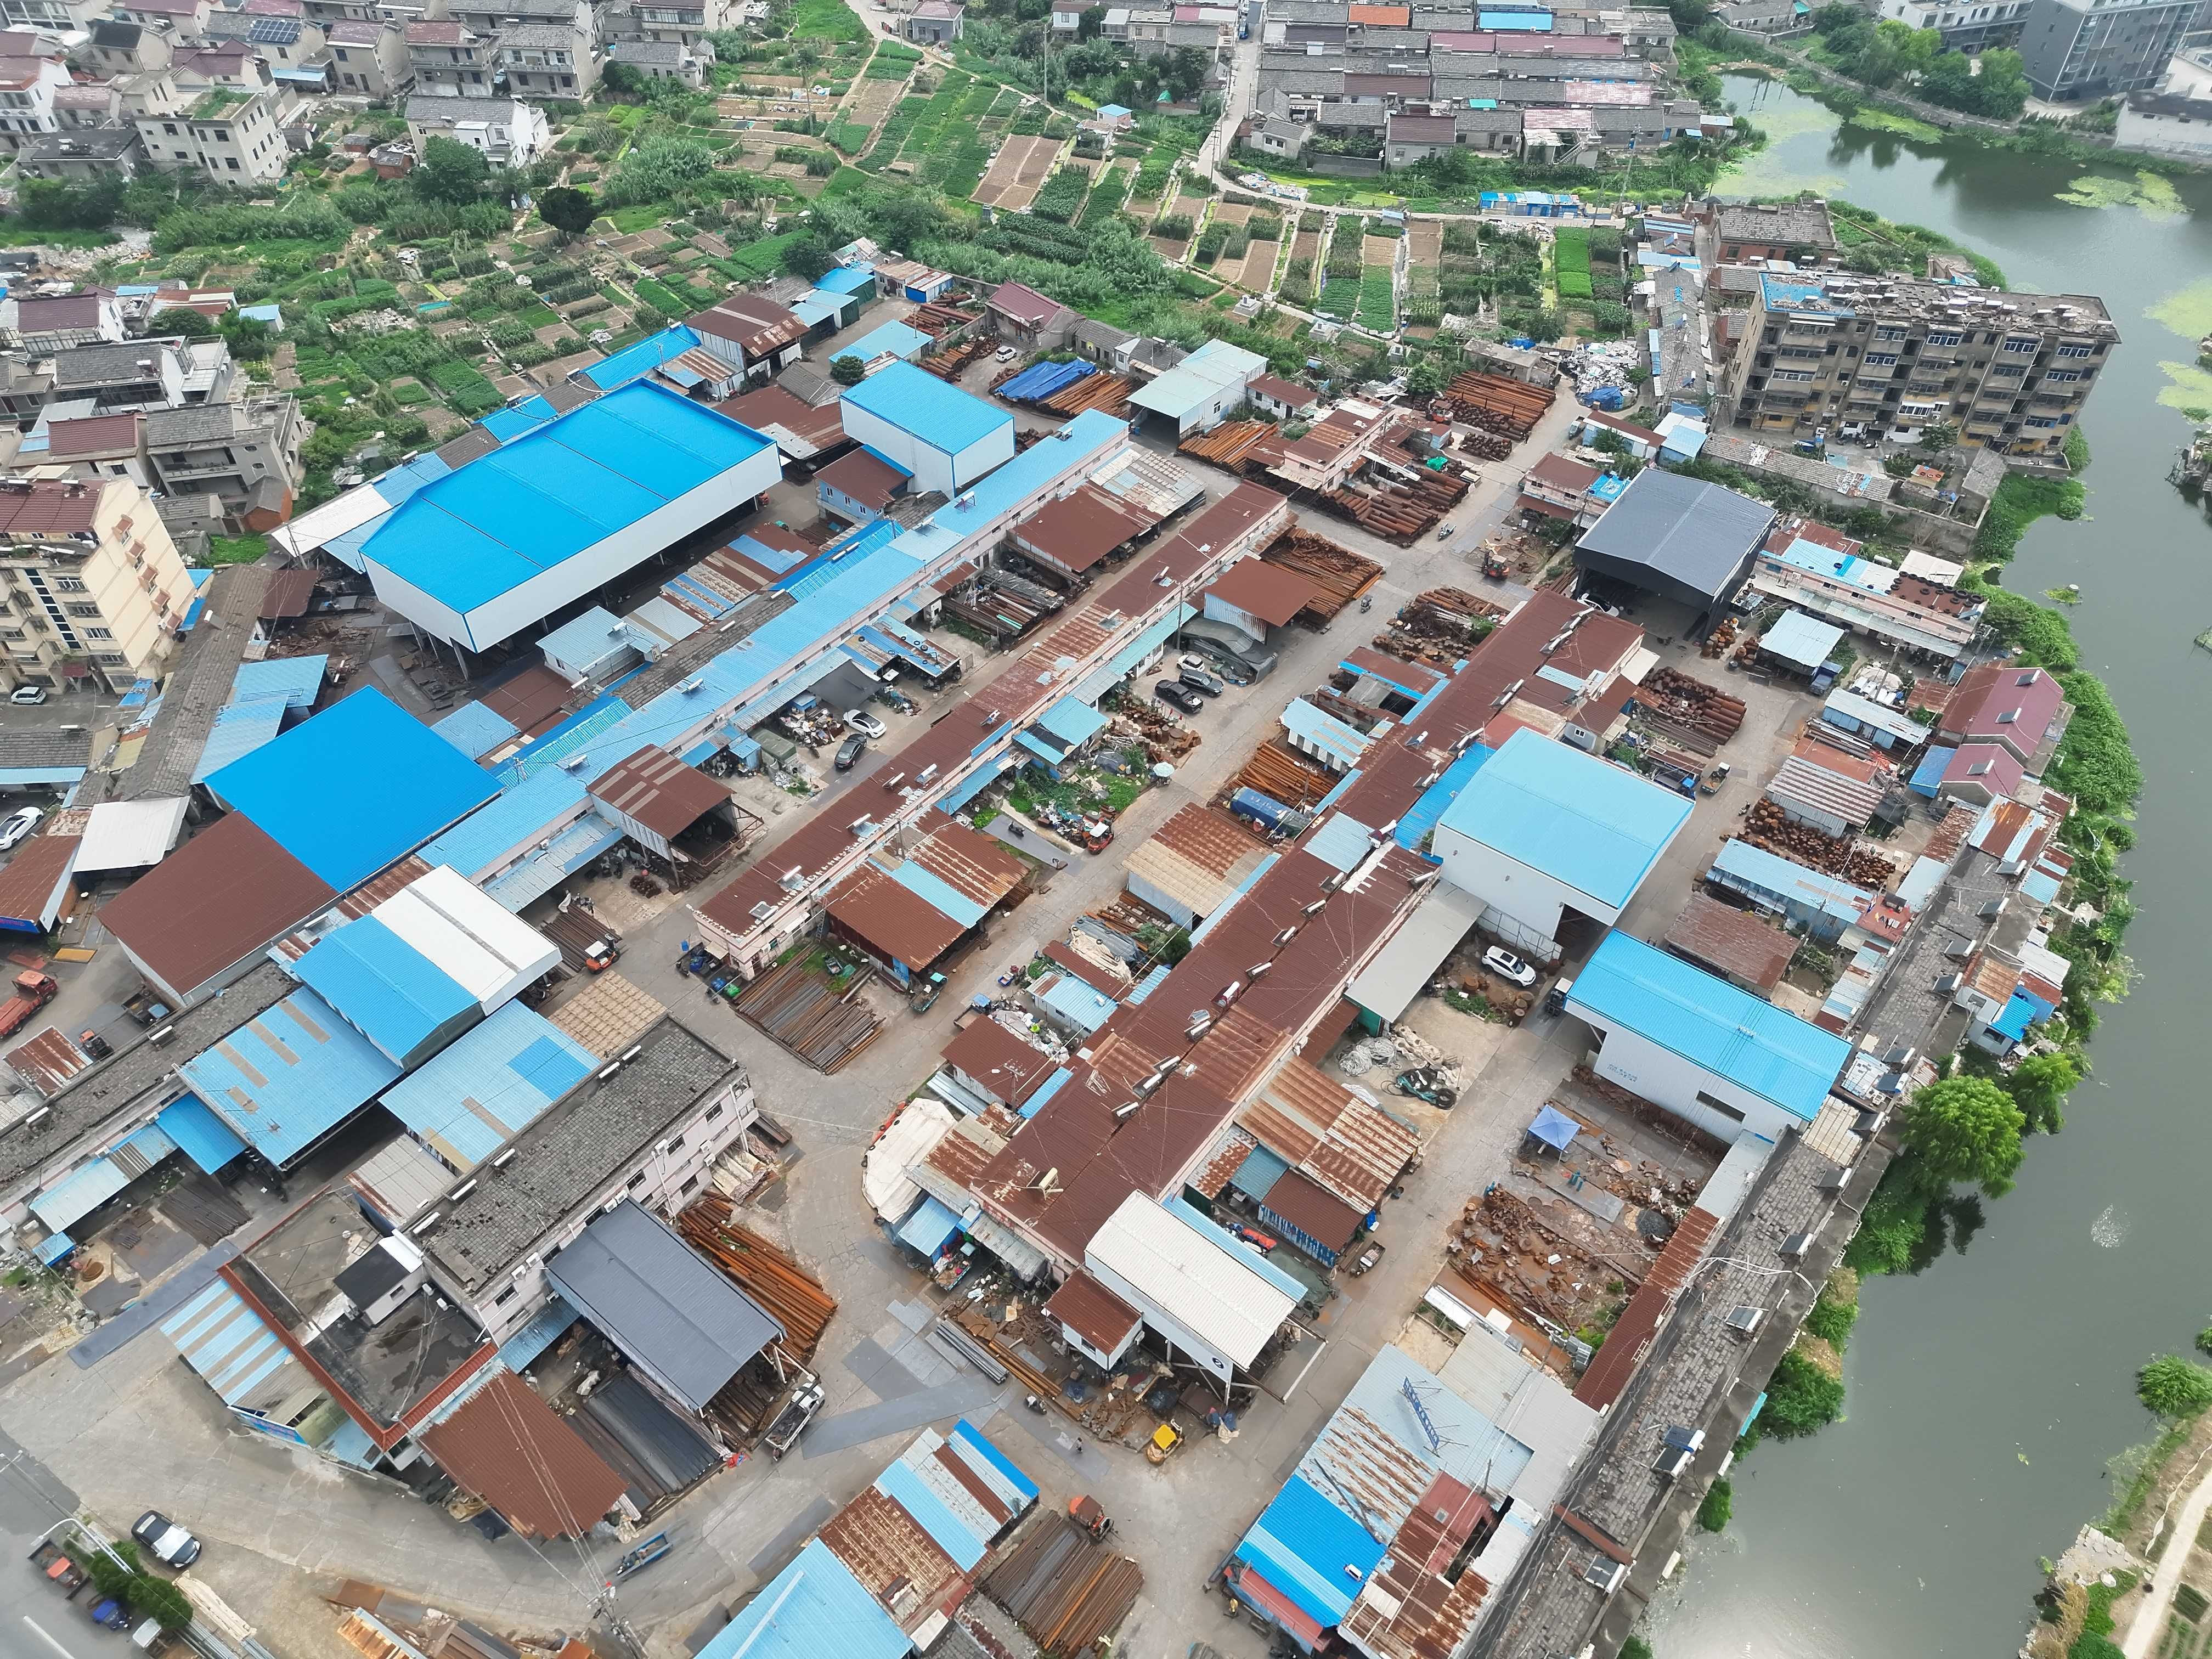
\includegraphics[width=0.61\linewidth,height=2.35cm,keepaspectratio]{construction_waste_context.jpg}\hfill
  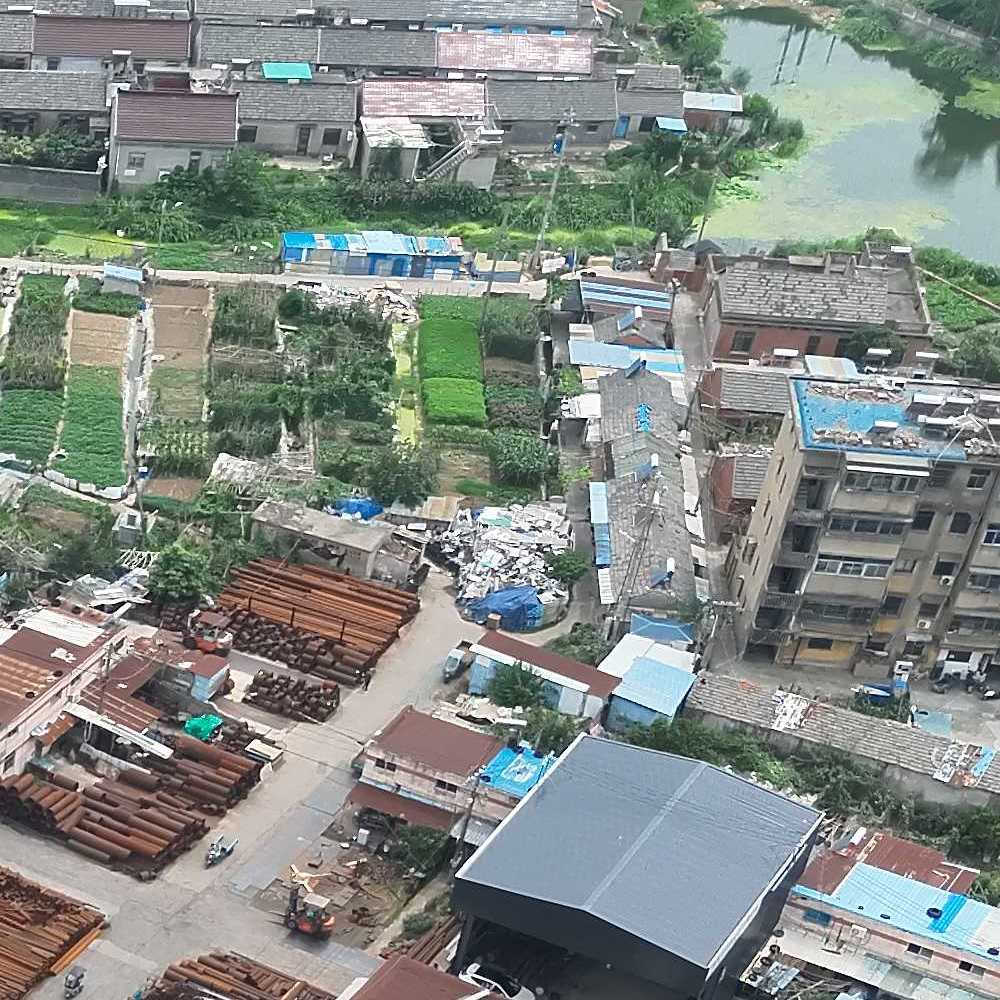
\includegraphics[width=0.37\linewidth,height=2.35cm,keepaspectratio]{construction_waste_evidence.jpg}
  \par\vspace{2pt}\footnotesize\textbf{(c) Construction waste.} Material, site context, and state interact.
\end{minipage}
\caption{Each annotation links a global context (left) to local evidence (right); exact-context grouping further joins multiple crops and events from the same scene. Operational labels require factor composition, not object naming. Images are internal examples pending release clearance.}
\label{fig:teaser}
\end{figure*}
